% !TEX encoding = UTF-8
% !TEX TS-program = pdflatex
% !TEX root = ../tesi.tex

%**************************************************************
\chapter{Web Service e Database}
\label{cap:sviluppo-software}
%**************************************************************

In questo capitolo sono trattati gli elementi di base delle soluzioni sviluppate. In primo luogo sono illustrati i Web Service responsabili della maggior parte delle operazioni. Successivamente è mostrato il Database di supporto con le principali caratteristiche.


%**************************************************************
\section{Web Service}

Secondo la definizione del \gls{W3C}, un Web Service è un sistema Software progettato per supportare l'interoperabilità tra diversi elaboratori su di una medesima rete.
Questa caratteristica si ottiene associando all'applicazione un'interfaccia Software che espone all'esterno i propri servizi, per mezzo della quale altri sistemi possono interagire con l'applicazione stessa utilizzando le operazioni descritte nell'interfaccia. L'utilizzo delle operazioni avviene tramite richieste, nel caso in esame di tipo SOAP (approfondito nella sezione \ref{soap}). I messaggi di richiesta sono formattati secondo lo standard \gls{XML}, incapsulati e trasportati tramite protocollo HTTPS. 
La connessione implementa il protocollo HTTPS, invece del classico HTTP, per aumentare la sicurezza del sistema, poiché trattandosi di dati riservati un utente malintenzionato vorrebbe poter disturbare la connessione o manomettere i dati trasmessi.\\
Grazie anche all'utilizzo di standard basati su XML, un'architettura basata su Web Service permette ad applicazioni Software scritte in diversi linguaggi di programmazione e implementate su diverse piattaforme Hardware di utilizzare le funzionalità che essa espone senza difficoltà.
\\Nella Figura \ref{webservice} è mostrato, in modo semplice, il funzionamento di un Web Service.

\begin{figure}[!h] 
    \centering 
    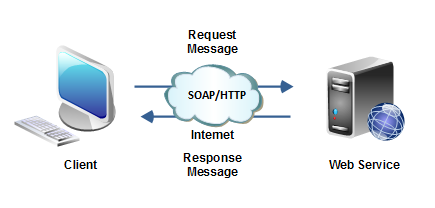
\includegraphics[width=0.60\columnwidth]{web-service} 
    \caption{Funzionamento di un Web Service.}
    \label{webservice}
\end{figure}


Nella realizzazione delle soluzioni sono stati sviluppati tre Web Service,\\ \texttt{LicenseManagerService}, \texttt{LicenseEmailService} e \texttt{LicenseSecurityService}, spiegati nei paragrafi successivi. Ognuno di essi è responsabile di funzionalità ben precise e sono indipendenti tra di loro per fornire un grado più alto di affidabilità ed eliminare le dipendenze.


\subsection{Richieste SOAP}
\label{soap}
SOAP, acronimo di \textit{Simple Object Access Protocol}, è un protocollo per lo scambio di messaggi tra componenti Software, nel caso in esame tra Client e Web Service, che avviene per mezzo della sintassi XML. \\
Il protocollo definisce un insieme di regole che il Client deve rispettare per richiedere al server che ospita ed espone il Web Service una determinata operazione.
\\
Un messaggio SOAP è formato da un \texttt{Header} e da un \texttt{Body}:
\begin{itemize}
\item \textbf{Header:} è facoltativo e contiene meta-informazioni, come ad esempio informazioni di sicurezza o parametri per eseguire una procedura;
\item \textbf{Body:} è obbligatorio e contiene il contenuto del messaggio, strutturato secondo l'\gls{XML Schema} imposto dal Web Service.
\end{itemize}

Nella Figura \ref{soap} è mostrato un esempio di richiesta e risposta del metodo \texttt{setEmail} del Web Service \texttt{LicenseEmailService}.

\begin{figure}[!h] 
    \centering 
    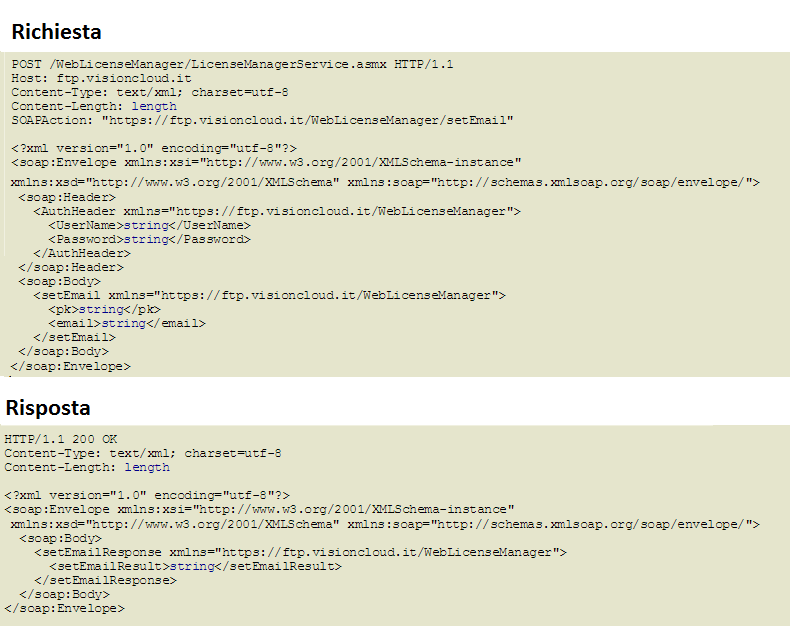
\includegraphics[width=1\columnwidth]{soap} 
    \caption{Esempio di richiesta e risposta SOAP.}
    \label{soap}
\end{figure}

Come si può vedere dalla Figura \ref{soap}, l'\texttt{Header} delle richieste è stato definito in modo da implementare un sistema di autenticazione per far sì che i Web Service siano utilizzati esclusivamente da Client autorizzati. Questo argomento è illustrato in dettaglio nel prossimo paragrafo.

\subsection{Autenticazione}
Per preservare la sicurezza dei dati ed evitare che chiunque possa utilizzare i servizi per la gestione delle licenze, è stato implementato un sistema di autenticazione per l'utilizzo dei Web Service. All'arrivo di una richiesta SOAP, i metodi controllano che sia presente l'Header (di norma opzionale), e che esso contenga gli elementi \texttt{UserName} e \texttt{Password}. Una volta verificata la loro esistenza, è invocata una funzione che verifica la validità delle credenziali in essi contenute. Se sono corrette il metodo continua la propria esecuzione, altrimenti ritorna un errore di autenticazione.

\subsection{LicenseManagerService}
\texttt{LicenseManagerService} è il Web Service che si occupa della gestione dei dati delle licenze e degli utenti di \textit{License Manager 1.0}, comunicando con il Database \texttt{DBLicenze} (illustrato nella sezione) per l'archiviazione e il ritiro dei dati. È il Web Service che fornisce più funzionalità, e coi suoi metodi riesce a supportare quasi la totalità delle operazioni richieste da \textit{License Manager 1.0}.\\
Le funzionalità più importanti da esso offerte sono:

\begin{itemize}
\item autenticare un utente per l'utilizzo di \textit{License Manager 1.0};
\item generare un \texttt{Product Key};
\item creare una licenza;
\item bloccare e sbloccare una licenza;
\item modificare la data di scadenza di una licenza;
\item eliminare una licenza;
\item disattivare una licenza;
\item fornire e modificare i moduli di una licenza;
\item restituire la lista delle licenze;
\item restituire la lista degli utenti di \textit{License Manager 1.0};
\item restituire la lista degli accessi al \textit{Software Gestionale Vision};
\item restituire l'insieme delle statistiche riguardanti le licenze;
\item gestire gli utenti di \textit{License Manager 1.0}.

\end{itemize}
 


\subsection{LicenseEmailService}
\texttt{LicenseEmailService} è il Web Service responsabile di gestire le operazioni legate agli indirizzi Email. La funzionalità più importante consiste nel generare un codice casuale e inviarlo tramite mail per verificare l'identità degli utenti e quindi autorizzare le operazioni più importanti. Questa procedura è svolta ad esempio nel momento della disattivazione di una licenza, dove si vuole controllare che l'utente operante sia lo stesso che l'ha attivata, avendo accesso all'indirizzo Email inserito in fase di attivazione. L'utente è quindi costretto a inserire lo stesso codice casuale inviato all'indirizzo Email associato alla licenza prima di poter continuare con l'operazione.\\
Di seguito sono riportate ulteriori funzionalità che il Web Service offre:
\begin{itemize}
\item restituire l'indirizzo email associato a una licenza;
\item restituire l'indirizzo email associato a un utente di \textit{License Manager 1.0};
\item notificare \textit{VISIONEIMPRESA s.r.l.} alla creazione di una licenza da parte di un rivenditore;
 \item notificare \textit{VISIONEIMPRESA s.r.l.} alla modifica di una licenza da parte di un rivenditore;
 \item inviare le credenziali di primo accesso a un nuovo utente di \textit{License Manager 1.0};
 \item inviare il \texttt{Product Key} da usare per una nuova attivazione in seguito alla disattivazione di una licenza.
\end{itemize}

\subsection{LicenseSecurityService}
\texttt{LicenseSecurityService} è il Web Service responsabile dei controlli da effettuare su una licenza e dell'area relativa alla sicurezza delle soluzioni sviluppate. La funzionalità più importante consiste nel verificare la validità di una licenza in termini di bloccaggio, data di scadenza e componenti Hardware. A un esito positivo il metodo responsabile ritorna una stringa contenente le informazioni da utilizzare per il controllo della validità di una licenza in modalità Offline. Il funzionamento dettagliato è affrontato nella sezione \ref{off}.
Per assicurare l'integrità dei messaggi scambiati col server, ove necessario, è utilizzato un sistema di cifratura a chiave pubblica, ad esempio per firmare i messaggi inviati dal server.\\
Le altre funzionalità che il Web Service offre sono:
\begin{itemize}
\item eseguire il controllo di una licenza durante l'esecuzione del \textit{Software Gestionale Vision}, affrontato nella sezione \ref{uniqueid};
\item restituire la chiave pubblica del server;
\item firmare digitalmente un messaggio con la chiave privata del server.

\end{itemize}


%**************************************************************
\section{Database}
\label{sez:DBLic}
Per l'archiviazione dei dati è utilizzato il Database relazionale \texttt{DBLicenze}, creato con SQL Server di Microsoft. L'ottenimento dei dati, per questioni di sicurezza, è affidato ai soli Web Service. Qualsiasi soluzione sviluppata deve affidarsi ai Web Service per interrogare il Database, aumentando il grado di affidabilità e riservatezza. L'utilizzo di un Database, in sostituzione al file condiviso tramite FTP, assicura maggiore consistenza dei dati, uso contemporaneo delle risorse grazie all'atomicità delle transazioni, controllo degli accessi, facilità nel reperimento dei dati e stabilità del sistema.


\subsection{DBLicenze}
Per raccogliere i dati relativi alla gestione e al controllo delle licenze è stato utilizzato un unico Database: \texttt{DBLicenze}. In seguito sono illustrate le tabelle che compongono il Database.

\subsubsection{Licenze}
È la tabella fondamentale contenente le licenze del \textit{Software Gestionale Vision}. \\Le informazioni in essa contenute, per ogni licenza, sono le seguenti:

\begin{itemize}
\item \texttt{Product Key};
\item \texttt{Serial Number};
\item \texttt{Tipologia};
\item componenti Hardware associate alla licenza. Esse sono espresse tramite una chiave esterna riferita alla tabella HWComponent;
\item eventuale blocco della licenza;
\item data di attivazione;
\item data di scadenza;
\item data di ultima attivazione;
\item numero di reinstallazioni;
\item data di ultimo accesso;
\item cliente;
\item email associata;
\item codice cifrato dei moduli;
\item codice dell'utente creatore;
\item autore del blocco, se presente;
\item data di creazione.
\end{itemize}

\subsubsection{Utenti}

Contiene gli utenti del Software \textit{License Manager 1.0}.\\ Le informazioni, per ogni utente, sono:

\begin{itemize}
\item username;
\item \gls{Hash} della password in \gls{SHA-256};
\item essere admin;
\item poter resettare la propria password;
\item codice utente (o codice rivenditore);
\item email associata all'utente.
\end{itemize} 

\subsubsection{HWComponent}

Contiene i dettagli dei computer che hanno o hanno avuto una licenza del \textit{Software Gestionale Vision} installata su di essi. \\Per ogni computer, le informazioni salvate sono:

\begin{itemize}
\item diverse componenti Hardware, non specificate per motivi di sicurezza;
\item Product Key della licenza associata;
\item data di attivazione della licenza;
\item data di disattivazione della licenza.
\end{itemize}

Alla disattivazione di una licenza il record relativo al computer da dissociare non è eliminato, ma rimane nella tabella impostando la data di disattivazione. In questo modo l'azienda è in grado di avere una panoramica completa sui PC in cui una licenza è stata installata, potendo notare possibili anomalie (ad esempio il ripetersi di installazioni sulle stesse macchine). 

\subsubsection{LicenseTransmittedID}

Contiene gli \texttt{UniqueID} utilizzati per il controllo durante l’esecuzione del \textit{Software Gestionale Vision} (riferirsi alla sezione \ref{uniqueid} per maggiori dettagli). \\Ogni record possiede le seguenti informazioni:

\begin{itemize}
\item \texttt{Product Key} della licenza a cui è associato l'\texttt{UniqueID};
\item \texttt{UniqueID} utilizzato per il controllo;
\item contatore delle risincronizzazioni effettuate;
\item eventuale permesso di risincronizzazione;
\item data e ora di creazione del record utilizzata per resettare il contatore delle risincronizzazioni ogni mese.
\end{itemize}

Il contatore delle risincronizzazioni è utilizzato per tenere traccia di quante volte l'\texttt{UniqueID} non viene trovato sul PC di cui verificare la validità della licenza. Esso può non essere trovato ad esempio per un'eliminazione involontaria dei file responsabili al controllo. Il numero di risincronizzazioni permesse è tre ogni mese, in seguito l'azienda è informata dell'anomalia.


\subsubsection{EmailCodice}

Contiene i codici inviati via Email per controllare l’effettivo possesso dell’indirizzo Email da parte degli utenti del \textit{Software Gestionale Vision}.
\\Ogni record possiede le seguenti informazioni:

\begin{itemize}
\item ID del codice da verificare;
\item indirizzo Email a cui è associato il codice;
\item codice da verificare;
\item data e ora di creazione del record per rendere inutilizzabile il codice dopo 10 minuti.
\end{itemize}

Ogni indirizzo Email può avere più codici in attesa di verifica (situazione causata dalla non ricezione delle mail che li contenevano), ma solo il più recente è ritenuto valido e utilizzato per il controllo. Inoltre, i codici generati da più di 10 minuti sono eliminati per questioni di sicurezza.

\subsubsection{LogAccessi}

Contiene gli accessi al \textit{Software Gestionale Vision}.
\\Ogni accesso ha le seguenti caratteristiche:

\begin{itemize}
\item ID dell'accesso;
\item \texttt{Product Key} della licenza di cui si registra l'accesso;
\item \texttt{indirizzo IP} dell'accesso;
\item \texttt{MAC Address} della scheda di rete del computer da cui si è effettuato l'accesso;
\item data dell'accesso;
\item codice utente associato alla licenza di cui si registra l'accesso.
\end{itemize}

Tra le informazioni è salvato anche il codice utente associato alla licenza per avere la lista degli accessi filtrabile per i diversi rifornitori.

\subsubsection{StoricoStatiLicenze}

Contiene gli stati passati di una licenza. Ogni stato è stato creato in seguito a una modifica. Lo stato attuale di una licenza è presente nella tabella \texttt{Licenze}.
\\Ogni stato è caratterizzato dalle informazioni variabili di una licenza, ed ha quindi le seguenti informazioni:

\begin{itemize}
\item ID dello stato;
\item componenti Hardware associate;
\item eventuale blocco;
\item data di scadenza;
\item cliente;
\item indirizzo Email;
\item codice cifrato dei moduli;
\item codice utente;
\item data di fine validità dello stato.
\end{itemize}

Disponendo di una tabella contenente gli stati di tutte le licenze antecedenti le modifiche l'azienda è in grado di avere una panoramica su tutto lo storico delle proprie licenze, evitando ad esempio equivoci con i rivenditori.